%----------------------------------------------------------------------------
%bb defines the bounding box for the pdf
%viewport defines the area of the pdf used
%in sidewaysfigure the last entry in bb moves the caption toward/away the pic
%in sidewaysfigure the second entry in bb moves the pic toward/away the caption
%----------------------------------------------------------------------------
\begin{figure}
\scalebox{0.8}[0.8]{
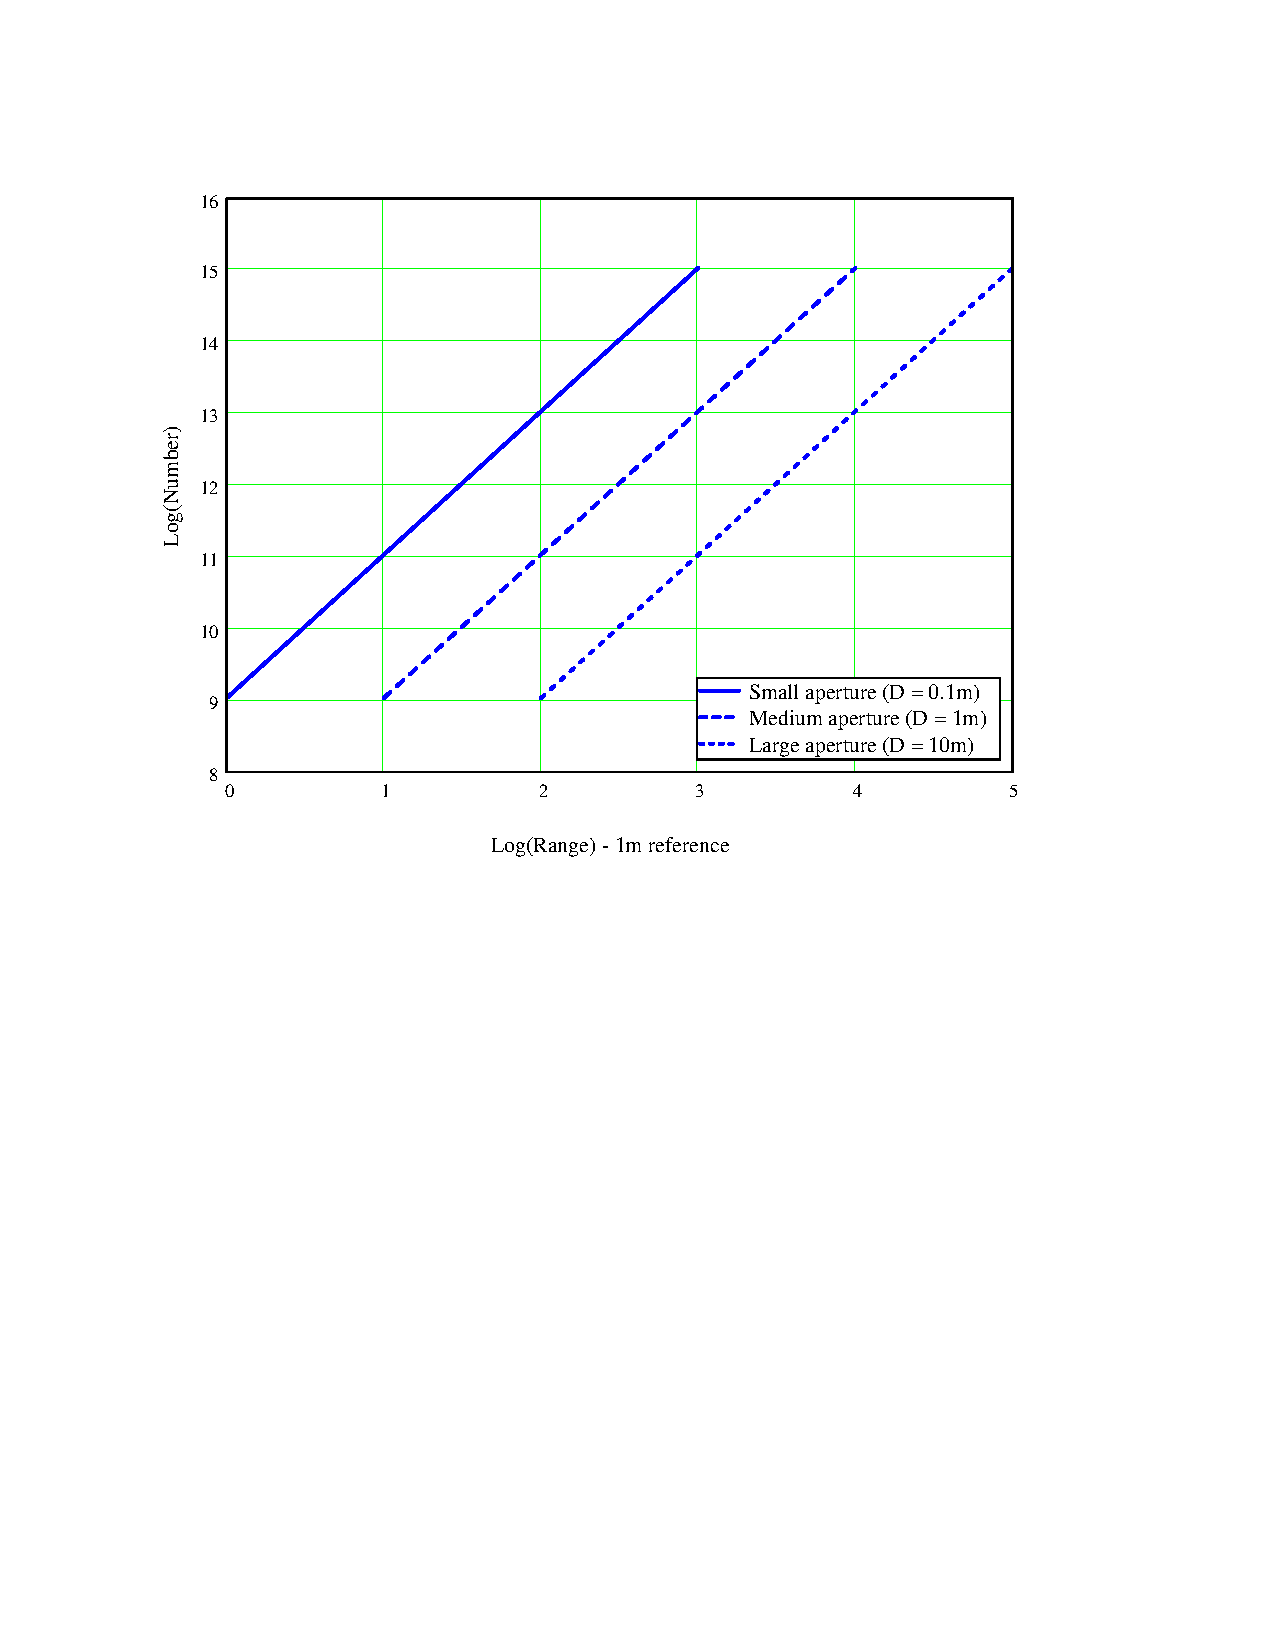
\includegraphics[bb=20 390 489 680]
{back_number/back_number.pdf}
}
\caption[Number of molecules emitting into reciever in a LIDAR application]{Number of molecules emitting into reciever acceptance area (ideal: $A=B=C=D\equiv1$ in Equation \ref{total_prob}). The ratio $R/D$ must be larger than unity to satisfy the approximations used to construct Equations \ref{energy_required} and \ref{v_eff}. Here we have used $\lambda=1$ $\mu$m, and a density of $10^{25}$ molecules per m$^3$. Thus, with an aperture of $D=1$ m and a focal length of 1 km, we expect the system to be sensitive to at most $10^{13}$ atmospheric molecules.}
\label{back_number}
\end{figure}
%----------------------------------------------------------------------------
